\vspace{-2mm}\section{Technical Approach}\vspace{-2mm}

% ? DK: Maybe break this down into sections


TVA will enable autonomous systems to more effectively and efficiently operate in new and uncontrolled environments through the use of several components. An overview of TVA is shown in Figure~\ref{fig:TVAOverview}, and its components are described below.


%which are described below and an overview is shown in Figure~\ref{fig:TVAOverview}. 


%\begin{figure}[h]
%	\centering
%     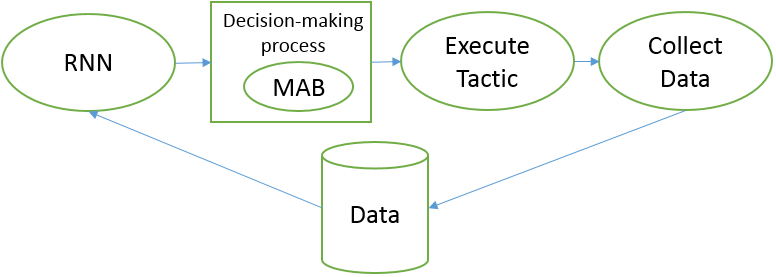
\includegraphics[width=0.8\linewidth]{images/Mab-Scratch.png}
%    \caption{TVA Process\dan{I will clean up - update}}
%    \label{fig:MABProcess}
%\end{figure}

%%%%%%%%%%%%%%%%% Start Image %%%%%%%%%%%%%%%%%%%%

\begin{figure}[h]

\begin{center}

%% Do this for right angles on connecting lines
\tikzset{
    -|/.style={to path={-| (\tikztotarget)}},
    |-/.style={to path={|- (\tikztotarget)}},
}

%% Rec, circle, rrec, arrow

\usetikzlibrary{fit, } %% Used for putting dotted box
\usetikzlibrary{calc}

\tikzstyle{line} = [draw, -latex']
\tikzstyle{arrow}=[draw, -latex] 
\
% Define block styles
\tikzstyle{line} = [draw, -latex']

\tikzstyle{circle} = [ellipse, draw, fill=white!20, text centered]

\tikzstyle{rrec} = [rectangle, draw, fill=white!20, text width=5em, text centered, rounded corners, minimum height=4em]

% Small rectangle
%\tikzstyle{smrrec} = [rectangle, draw, fill=white!20, text centered, maximum height=2em]

% Database icon
\tikzstyle{dbase} = [cylinder, draw, fill=white!20, shape border rotate=90, minimum height=3em, minimum width=1.45cm]

\scalebox{.9}{
\begin{tikzpicture}[node distance = 3.5cm, line width=.5mm]
   
    \node [dbase] (Data) {Data}; 

    \node [circle, above left of=Data, yshift=0ex, xshift=3ex, maximum height=1em, maximum width=.5em] (MAB) {MAB}; %was 3 yshift

    \node [rrec, left of=MAB] (RNN) {RNN};
    \node [rrec, right of=MAB] (Execute) {Execute Tactic(s)};
    \node [rrec, right of=Execute] (Collect) {Collect Tactic Data};

    \draw [line] (RNN) -- (MAB);
    \draw [line] (MAB) -- (Execute);
    \draw [line] (Execute) -- (Collect);
    \draw [line] (Data) -- (RNN);
    \draw [line] (Collect) -- (Data);

    \draw[black,thick] ($(MAB.north west)+(-.65,0.5)$) rectangle ($(MAB.south east)+(0.65,-0.5)$) ++(-1.3,2.2) node[below] {Decision Process};

\end{tikzpicture}
} 
\caption{Overview of TVA process}
\label{fig:TVAOverview}
\end{center}
\end{figure}

%%%%%%%%%%%%%%%%% End Image %%%%%%%%%%%%%%%%%%%%

\vspace{-5mm} % Will likely need to be adjusted

\begin{enumerate}[noitemsep]

    \item \descStep{Use RNNs to Predict Tactic Values}{Tactic attributes such as latency and cost will be predicted using the Evolutionary Exploration of Augmenting Memory Models (EXAMM) algorithm. % to evolve RNNs to predict time series data from system \hl{sensors}. 
    We will further extend \hl{?existing?} EXAMM-based methods to utilize not only mean squared error (MSE) and mean absolute error (MAE) of predictions as loss functions, but also incorporate a measure of confidence -- predicting an estimation of running standard deviation for the time series.\dan{Travis: Update}}    

    \item \descStep{Plan for Tactic Execution With Multi-Armed Bandit Approach}{The inclusion of a multi-armed bandit component will augment the system's decision-making process, and better enable the system to explore and select between multiple tactic options. The multi-armed bandit component will be especially beneficial for providing additional tactic data, especially in situations of high uncertainty/volatility and when there are little amounts of historical tactic data. %For example, consider a scenario where the system has two tactic options with equal reward, but volatile cost and latency. To enable the system to regularly gain updated cost and latency information, it is necessary to regularly `explore' the alternative tactic option to understand its updated cost information. Not exploring alternative tactic options could lead to scenarios where the system `learns' to always choose one of the tactic options, when in fact an alternative tactic option has become cheaper and/or faster. Therefore, the system would lose the opportunity to begin to utilize this alternative, more optimal tactic. 
    A challenge is to balance the `explore' and `exploit' components for the system to optimally function. While the specific implementation remains to be evaluated and determined, options include Epsilon Greedy or Upper Confidence Bound approaches. Specific domain and system requirements will heavily influence the possible influence that the multi-armed bandit component has on the system. In cases of high uncertainty or low confidence, the system may execute an appropriate \emph{uncertainty reduction tactic}~\cite{moreno2018uncertainty}
    
    
    
    
    %to exploit and explore tactic option(s) when appropriate. 
    
    
    % Briefly explain the benefits that MAB will provide.
    % Tactic predictions need further data
    
    % For example, consider a scenario where the system has two tactic options with equal reward, but volatile cost and latency. To enable the system to regularly gain updated cost and latency information
    
    
    % Not exploring alternative tactic options could lead to scenarios where the system `learns' to always choose one of the tactic options, when in fact an alternative tactic option has become cheaper and/or faster. Therefore, the system would lose the opportunity to begin to utilize this alternative, more optimal tactic. 
    
    
    }
    
    %The system will plan for tactic execution(s) using a multi-armed bandit component. This will enable the system to effectively perform, while also accounting for volatility, uncertainty and a lack of empirical data. While the specific implementation remains to be evaluated and determined, several initial options include Epsilon Greedy or Upper Confidence Bound approaches. Specific domain and system requirements will heavily influence the possible `exploration' that is conducted by the selected multi-armed bandit approach. In cases of high uncertainty or low confidence, the system may execute an appropriate \emph{uncertainty reduction tactic}~\cite{moreno2018uncertainty}.}
    
    %Plan for Tactic Execution Using Multi-Armed Bandit Approach}{Existing knowledge, system rules and the results from the RNN model will be incorporated into our decision-making process which a significant Multi-Armed Bandit component. This will enable the system to not only account for the predicted tactic, but also account for predicted tactic confidence and variance. This multi-armed bandit approach, coupled with the use of evolutionary RNNs will enable the system to most appropriately function in new and uncontrolled areas, and especially those with volatile or small amounts of historical data.\todo{work on this section}}
    
    % Help in scenarios where little information is known
    % Assist when there isn't much confidence about a predicted value
    % ? Which MAB process will we use.
    
    % Combine with the RNNs results along with system/domain-specific requirements to determine the most appropriate tactics to implement.
    
    % Provide more specifics about how we plan to use MABs
    
    
    
%    \item \descStep{Plan for Tactic Execution}{The Multi-Armed Bandit component will determine the most appropriate tactic(s) to execute.}
    
    
    \item \descStep{Execute Tactics}{Tactics are executed according to defined plan.}



    \item \descStep{Collect Tactic Data}{System sensors record the amount of time and cost required to execute the adaptation tactic(s). Other relevant time series data will also be collected by the system throughout its operation. This data will also be included in future tactic-based predictions.}




%    \item \descStep{Collect tactic values}{XXXXX}
%    \item \descStep{Make prediction for latency, cost, \etc}{XXXXX}
%    \item \descStep{Put prediction back into decision-making process}{XXXXX}



\end{enumerate}



%%%%%%%%%%%%%%%%%%%%%%%%%%%%%%%%%

%Our proposed TVA solution will benefit a variety of autonomous systems through its easy integration into a diverse forms of self-adaptive processes. (HOW)..... 


%TVA will enable autonomous to better react to tactic volatility using the following processes:





%Can impact adaptation tactics, along with adaptation strategies which are predefined compositions of adaptation tactics~\cite{moreno2017adaptation}.



%decision trees built out of adaptation tactics~\cite{moreno2017adaptation}.

%\begin{enumerate}[noitemsep]

%    \item \descStep{Collect tactic values}{XXXXX}
%    \item \descStep{Make prediction for latency, cost, \etc}{XXXXX}
%    \item \descStep{Put prediction back into decision-making process}{XXXXX}
%    \item \descStep{XXX}{XXXXX}


%\end{enumerate}



% DK: I think that these are good, but are also a bit too technical and miss several important details.
%Our TVA process will consist of several primary phases which are described below:

%\begin{enumerate}[noitemsep]

%\item \descStep{Predict Tactic Volatility}{We will use the Evolutionary Exploration of Augmenting Memory Models (EXAMM) algorithm to evolve RNNs to predict time series data from system \hl{sensors}. We will further extend EXAMM to utilize not only mean squared error (MSE) and mean absolute error (MAE) of predictions as loss functions, but also incorporate a measure of confidence -- predicting an estimation of running standard deviation for the time series.}

%\item \descStep{Bootstraping Trained RNNs to New Scenarios and Data}{We will investigate the use of using previously trained RNNs and evolving them to quickly predict new parameters with limited available data, for example, if a new sensor system becomes available; or re-evolve a network if sensors are damaged and become unavailable.\dan{we should add in a few words how this fits into TVA better.}}

%\item \descStep{Incorporate predictions into decision-making process}{The anticipated tactic volatility values will be incorporated into the decision-making processes in several ways. The estimated tactic values can be used to make more accurate predictions for what the attained \emph{utility} of a specific tactic will be. This can in turn, impact the expected utility of the larger \emph{adaptation strategies} that the system may take. The anticipated tactic latency times will enable the system to more accurately determine when tactics should be proactively began to ensure that they are ready when needed, thus improving system effectiveness and reducing cost due to the system realizing less waste with tactics enacted before they are needed. The latency values will also be used by the system to make more informed decisions about how different tactics and adaptation strategies will impact concurrent and subsequent tactics and adaptation strategies.}



%The calculated confidence and variance of parameters in the tactic predictions can provide even further data points that the system can incorporate into its decision-making process. For example, if a tactic prediction has a low amount of confidence, the system could choose to execute an \emph{uncertainty reduction tactic}~\cite{moreno2018uncertainty} to potentially provide a more accurate prediction.\dan{move}



%The estimated tactic values will be included in the system's \emph{utility} equation which is often used to guide the system's actions and the decisions-made by the system. The estimated values will also be \hl{compared} with the specifications defined in the SLA to enable the system to act more proactively when necessary to ensure that the specifications defined in the SLA are adhered to.\dan{rewrite this}\dan{make sure that this is all accurate}}

% DK: Be sure that I am using adaptation tactic and adaptation strategy correctly here.


%The estimated tactic values will be included in the system's decision-making process, enabling it to make more informed decisions leading to more optimal outcomes.


%% DK: I am not sure that this step is actually needed since it is kind of explained in the previous step
%\item \textbf{Perform system operations using predictions: }The input values will enable the system to make more appropriate and informed actions, thus supporting it in dynamic and volatile environments. \dan{rewrite this}
	
%\end{enumerate}

%\dan{ALL: Does this provide enough information/confidence for how this will actually work?}



% Provide the reader confidence in how all of this comes together

% Process of how TVA works collected tactic information, learning, prediction, action. 
%   Where is it integrated to in the MAPE-K control loop. 

% Provide a lot of confidence for how it will be integrated into the self-adaptive process
% Talk about why RNN is the most appropriate solution here. Provide confidence. Also, discuss a bit about how RNN works

% Mention how it will integrate into a variety of autonomous systems (either here or in another section of the paper)



% In systems that do not directly utilize a SLA, the improved tactic estimations can still be used to benefit the decision-making process of these systems by providing more informed and accurate tactic attribute values. Future work should be conducted to examine precisely how our TVA process can be incorporated into these systems and determine the benefits that they will have.



%\subsection{--- ML and how it will fit into this project ----}

%\dan{Travis/Qi/Alex: this is your section}

% What is the process we will use
% Why will it be the most effective from a technical perspective. 
% What are some things that make it innovative/interesting.



% DK: Provide the reader confidence in why the ML techniques we are choosing will be proper. Don't be afraid to be a bit innovative here.





% DK: Probably cut down on this space a bit more in the event space is needed. I think that this section is less important that most of the others.
\subsection{Evaluation Process}

% Describe how it will be evaluated using different tools, different data sets. Make the reader confident in the need to create our own dataset.

We will evaluate our proposed TVA processes against the defined objectives using our created dataset containing real-world tactic volatility using statistical evaluations such as R and MatLaB, and in the existing simulation environments SWIM~\cite{moreno2018swim} and DARTSIM~\cite{MorenoDART2019}. %\dan{Add in how R, MatLab will be used.}
To support the evaluation of TVA, enhancements to DARTSim and SWIM will include support for volatile data, additional scenarios, and new adaptation tactics and strategies. The effectiveness of our proposed TVA solution will be evaluated using several metrics including: (I) Expected vs realized utility (II) Ability to complete defined mission/system critical functionality when encountering unexpected volatility and when operating in new environments (III) Ability of TVA to assist the system's ability to execute concurrent and subsequent adaptation tactics and strategies (IV) Speed of learning..... ???   .\dan{What more can we add to these?}

%To evaluate our work, we will utilize several scenarios, including the cloud-based example described in Section~\ref{sec: motivatingexample} and the UAV scenario provided in DARTSim.






%The effectivness to:
%-   execute si


% How and why we will need to modify the tools
% What metrics will we use evaluate the techniques.
% What scenarios will we use (use the existing cloud-based or come up with a military scenario)
 



% Train in different environments
% Cut out sensors
% Different systems

 



\todo{How will we evaluate the ML portion}

We will evaluate various multi-armed bandit solutions (\eg Epsilon-Greedy, Upper Confidence Bound, Bayesian) to assess their effectiveness in various autonomous environments and scenarios.